\documentclass[11pt]{article}
\usepackage[margin=0.9in]{geometry}
\usepackage[T1]{fontenc}
\usepackage{lmodern,microtype,booktabs,float,xcolor,enumitem,tabularx,array}
\usepackage{tikz,pgfplots}
\usetikzlibrary{arrows.meta,positioning,shapes.geometric}
\pgfplotsset{compat=1.18}
\usepackage{adjustbox}
\usepackage[hyphens]{xurl}
\usepackage[hidelinks]{hyperref}
\setlist{itemsep=2pt,topsep=3pt}
\newcommand{\num}[1]{\textbf{#1}}
\definecolor{ember}{HTML}{C2410C}
\title{\textbf{Emberz}: a fine-tuned guardian model for live phone-call safety\\[2pt]\large Fireworks: Deploy Buildathon with Microsoft \& NVIDIA}
\author{Matt Ceran \and Numan Karakas}
\date{San Francisco, November 2, 2026}
\begin{document}
\maketitle

\begin{abstract}
\noindent \textbf{Emberz gives a child, a grandparent or any vulnerable person a guarded phone number.} Every call from an unknown number is transcribed live, and a model \emph{fine-tuned on Fireworks} scores each turn. It stays silent on normal calls. When a call turns into a scam, a stranger fishes a child for personal information, a grooming tactic appears, or a caretaker's own written rule is broken, it whispers a coaching line to the protected person, alerts the caretaker (who can listen in and join), and shows the live transcript on a caretaker console.
On 257 held-out calls written by a different model family than the training data, our fine-tuned Qwen3.6-35B-A3B guardian (v2) catches \num{92.6\%} of risky calls \emph{before the scammer's ask} and false-alarms on \num{17.7\%} of harmless look-alike calls, against 53.2\% for the same model untuned, 38.0\% for Fireworks' Rune, 31.6\% for DeepSeek V4.1 Flash and 22.8\% for Kimi K3. It gets \num{19 of 22} caretaker-rule pairs right; every baseline gets 5 or fewer. Counting every call, it handles \num{90.3\%} correctly against 75.5\% untuned and 83.7\% for Kimi K3, and McNemar's test and a scenario-clustered bootstrap confirm every gain ($p \le 0.005$). On BothBosu, a public dataset from another model family, it catches 98 of 100 scams with zero false alarms.
\end{abstract}

\section{The problem and why it matters}
\begin{itemize}
\item \textbf{Elder fraud.} Americans aged 60+ reported \$7.7B in losses in 2025 (FBI IC3~\cite{ic3}), with an average loss near \$38.5K; imposter scams alone accounted for \$3.5B (FTC~\cite{ftc}). Phone calls are the main vector: bank and government impersonation, tech support, grandparent and family-emergency scams, crypto and romance.
\item \textbf{Children.} Online-enticement reports to NCMEC rose 158\% to 1.4M in 2025~\cite{ncmec}. Grooming follows recognizable \emph{tactics}: flattery and gifts, secrecy requests, moving to another app, asking whether parents are home or which school, photo and meeting requests.
\item \textbf{The gap.} Existing tools (on-device scam detection on Pixel and Galaxy phones, Hiya, Truecaller, OnGuardAI) are scam-only, warn only the person being manipulated, or check the voice only. We found none that streams a live call to a caretaker under rules the caretaker writes, or that covers children's calls.
\end{itemize}

\begin{figure}[H]\centering
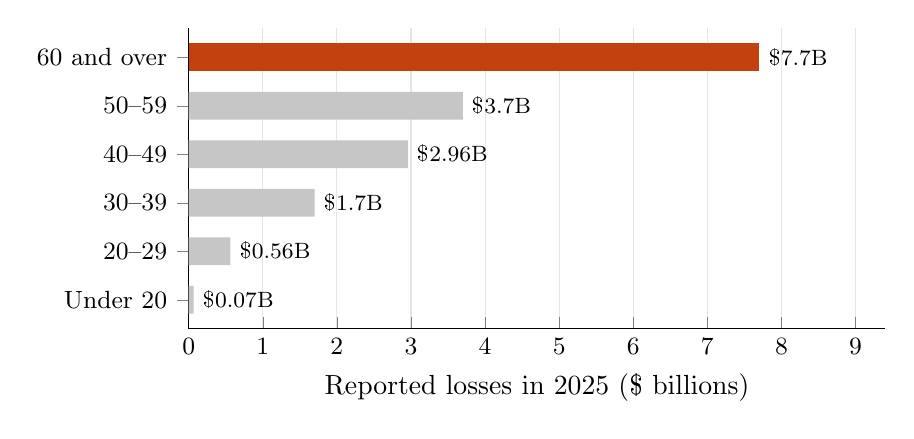
\begin{tikzpicture}
\begin{axis}[xbar, bar shift=0pt, width=0.86\linewidth, height=5.4cm, bar width=10pt, xmin=0, xmax=9.4,
  symbolic y coords={Under 20,20--29,30--39,40--49,50--59,60 and over}, ytick={Under 20,20--29,30--39,40--49,50--59,60 and over},
  xlabel={Reported losses in 2025 (\$ billions)}, axis x line*=bottom, axis y line*=left,
  xmajorgrids, grid style={gray!20}, enlarge y limits=0.12, tick label style={font=\small},
  nodes near coords={\$\pgfmathprintnumber[fixed,precision=2]{\pgfplotspointmeta}B}, nodes near coords align=horizontal,
  every node near coord/.append style={font=\footnotesize}]
\addplot[fill=gray!45, draw=none] coordinates {(0.067,Under 20) (0.563,20--29) (1.7,30--39) (2.957,40--49) (3.7,50--59)};
\addplot[fill=ember, draw=none] coordinates {(7.7,60 and over)};
\end{axis}
\end{tikzpicture}
\caption{Older Americans lose the most. Reported fraud losses by victim age in 2025. People 60 and over filed 20\% of the 1,008,597 complaints but lost \$7.7B, 37\% of the \$20.9B total, about \$38{,}300 per complaint. Losses overall rose 26\% from 2024. Source: FBI IC3 2025 Annual Report~\cite{ic3}.}\label{fig:ic3}
\end{figure}

\begin{table}[H]\centering\small
\caption{The call-driven scams Emberz targets, and what preventing a share of them is worth. Losses are the FBI IC3 2025 figures~\cite{ic3}; the prevention rows are arithmetic on those totals.}\label{tab:addressable}
\begin{tabular}{lr}\toprule
Crime type (FBI IC3, 2025) & Reported losses \\ \midrule
Tech support & \$2.13B \\
Confidence and romance & \$0.93B \\
Government impersonation & \$0.80B \\ \midrule
\textbf{Addressable losses} & \textbf{\$3.86B a year} \\ \midrule
Every 1\% prevented & \$38.6M a year \\
5\% prevented & \$193M a year \\
10\% prevented & \$386M a year \\
\bottomrule\end{tabular}\end{table}

\noindent\textbf{Where Emberz intervenes.} The money moves at the \emph{ask}: the moment the caller asks for the code, the transfer or the gift cards. In our evaluation the guardian alerts before that moment on \num{92.6\%} of risky calls, a median of \num{4.5 turns} early. That is the window in which a private coach line or a caretaker joining the call can stop the payment. For children, IC3 received more than 75,000 sextortion reports~\cite{ic3} in 2025, 11,316 of them from people under 20, and most began with someone posing as a peer; Emberz flags the grooming tactics that come first.

\subsection*{AI callers raise the stakes}
AI makes these calls cheaper to run and harder to spot. IC3~\cite{ic3} counted \num{22,364} fraud complaints mentioning AI in 2025, with \num{\$893M} in losses, and warns that AI-made voices and scripts are ``increasingly difficult to detect and easier to make''. Voice cloning now powers ``distress'' scams in which a loved one's voice begs for money. The losses per victim are far larger when AI is involved:

\begin{figure}[H]\centering
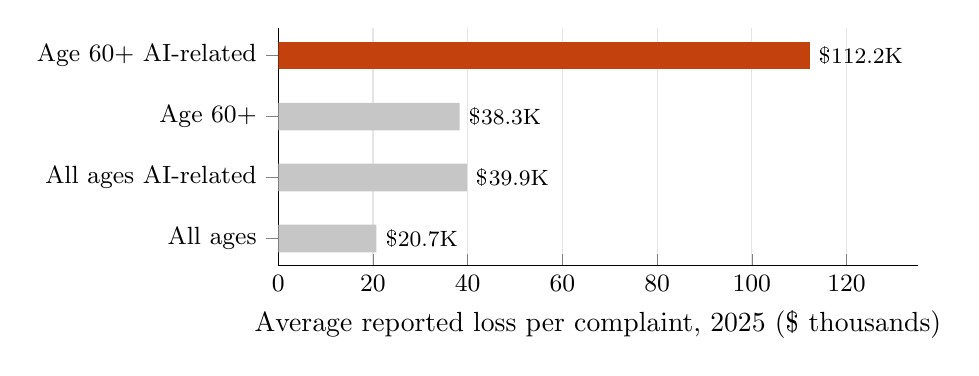
\begin{tikzpicture}
\begin{axis}[xbar, bar shift=0pt, width=0.8\linewidth, height=4.6cm, bar width=10pt, xmin=0, xmax=135,
  symbolic y coords={All ages,All ages AI-related,Age 60+,Age 60+ AI-related},
  ytick={All ages,All ages AI-related,Age 60+,Age 60+ AI-related},
  xlabel={Average reported loss per complaint, 2025 (\$ thousands)}, axis x line*=bottom, axis y line*=left,
  xmajorgrids, grid style={gray!20}, enlarge y limits=0.15, tick label style={font=\small},
  nodes near coords={\$\pgfmathprintnumber[fixed,precision=1]{\pgfplotspointmeta}K}, nodes near coords align=horizontal,
  every node near coord/.append style={font=\footnotesize}]
\addplot[fill=gray!45, draw=none] coordinates {(20.7,All ages) (39.9,All ages AI-related) (38.3,Age 60+)};
\addplot[fill=ember, draw=none] coordinates {(112.2,Age 60+ AI-related)};
\end{axis}
\end{tikzpicture}
\caption{AI-related fraud costs older victims about 3$\times$ more per complaint. Averages computed from FBI IC3 2025 totals~\cite{ic3}: all complaints \$20.877B / 1,008,597; AI-related \$893.3M / 22,364; people 60+ \$7.7B / 201,266; AI-related from people 60+ \$352.5M / 3,143. People 60+ account for 39\% of all AI-related losses.}\label{fig:ai}
\end{figure}

IC3 also notes these figures are a floor: investment complaints with a reported AI link passed \$632M, while investment losses overall exceeded \$8B, ``demonstrating that many victims do not realize the extent AI may be involved''. Emberz checks the caller's voice in the first 2--4 seconds of the call. Our AI-voice detector, trained and tested on the In-the-Wild deepfake dataset~\cite{itw}, catches 98\% of AI clips at a 1\% false-alarm rate on speakers it never saw, through a simulated phone line, and an AI voice from an unknown number that asks for money, a code or personal information goes straight to an alert.

\section{What we built}
\subsection{Product}
A caretaker gives the protected person a \textbf{guarded Telnyx number}. Calls from saved contacts are still checked against the caretaker's rules, but judged more leniently. Unknown callers hear a short notice (``this call is protected and may be transcribed''), then the call is bridged to the protected person's real phone while both sides of the audio stream to our line server. The \textbf{caretaker writes rules in plain words} (``never share the door code'', ``alert me about any talk of money, even with family'').

\subsection{System}
\begin{center}
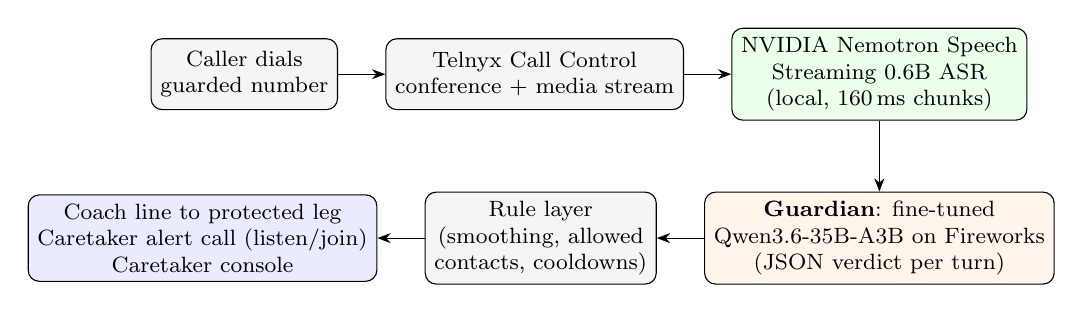
\begin{tikzpicture}[node distance=5mm and 6mm, box/.style={draw,rounded corners,align=center,font=\footnotesize,minimum height=9mm,fill=#1!8}, box/.default=gray, >=Stealth]
\node[box=gray] (c) {Caller dials\\guarded number};
\node[box=gray, right=of c] (t) {Telnyx Call Control\\conference + media stream};
\node[box=green, right=of t] (a) {NVIDIA Nemotron Speech\\Streaming 0.6B ASR\\(local, 160\,ms chunks)};
\node[box=orange, below=9mm of a] (gd) {\textbf{Guardian}: fine-tuned\\Qwen3.6-35B-A3B on Fireworks\\(JSON verdict per turn)};
\node[box=gray, left=of gd] (p) {Rule layer\\(smoothing, allowed\\contacts, cooldowns)};
\node[box=blue, left=of p] (o) {Coach line to protected leg\\Caretaker alert call (listen/join)\\Caretaker console};
\draw[->] (c)--(t); \draw[->] (t)--(a); \draw[->] (a)--(gd); \draw[->] (gd)--(p); \draw[->] (p)--(o);
\end{tikzpicture}
\end{center}
\begin{itemize}
\item \textbf{Speech-to-text:} NVIDIA Nemotron Speech Streaming 0.6B~\cite{nemospeech} (INT8, sherpa-onnx) on a laptop: 34\,ms compute per 160\,ms chunk for both call sides together, 0--2\% WER on short clean 8\,kHz TTS probes (15.9\% median WER on 49 full test calls, mostly numbers written as words). It runs locally next to the line server.
\item \textbf{Guardian:} reads the protected person's profile, the caretaker's rules, whether the caller is a saved contact, an AI-voice signal, its own previous verdict and the last 8 turns, then returns one JSON verdict per turn:
\texttt{\{risk: none|watch|alert|urgent, category, severity, source, stage, evidence[\{turn, quote\}], action, coach\_line, caretaker\_note\}}.
Categories: 5 scam types, 4 disclosure types (location/school, codes/passwords, financial IDs, home alone), 5 grooming tactics, vulgar, threat/extortion, self-harm, \texttt{custom\_rule} (a caretaker rule broken) and none.
\item \textbf{Console:} a phone-friendly caretaker page with the live transcript of both sides, a risk meter, the alert note with the quoted evidence, the coach line, and Listen / Join / Hang up / Mark safe. It also replays synthetic held-out test calls with the model's actual recorded verdicts.
\end{itemize}

\subsection{AI-voice detection}
The line scores the first 2--4 seconds of the caller's speech for a synthetic voice and passes the score to the guardian with every turn. An AI voice alone is at most \emph{watch} (a pharmacy reminder bot is fine); an AI voice from an unknown number that asks for money, a code or personal information escalates to an alert.
\begin{itemize}
\item \textbf{Model:} frozen \texttt{facebook/wav2vec2-xls-r-300m} features (hidden states of layers 3, 6, 9 and 12, mean and standard deviation pooled, 2,048 dimensions), then standardization, logistic regression and Platt calibration. Layer 9 and $C=1.0$ were picked on held-out dev speakers.
\item \textbf{Data:} a balanced 5,998-clip subset of In-the-Wild~\cite{itw} (real and deepfake speech of public figures), split \emph{by speaker} so no test speaker appears in training. Every clip goes through the live line's phone path (8\,kHz G.711 $\mu$-law) and the same speech gate the line uses, which drops leading silence.
\item \textbf{Speed:} 33\,ms to score a 4-second clip; the live detector scores 20\,ms phone frames as they arrive.
\end{itemize}
\begin{table}[H]\centering\small
\caption{AI-voice detector on 2,829 clips from 25 speakers it never saw (1,413 AI, 1,416 human). 95\% intervals from a class-stratified bootstrap.}\label{tab:voice}
\begin{tabular}{lcc}\toprule
Test condition & Equal error rate & ROC AUC \\ \midrule
\textbf{Phone path, first 4\,s of speech} & \textbf{1.27\%} \scriptsize(0.85--1.77) & \textbf{0.9991} \scriptsize(0.9985--0.9996) \\
Phone path, first 2\,s (the live early check) & 1.55\% \scriptsize(1.06--2.05) & 0.9988 \scriptsize(0.9979--0.9994) \\
Clean audio, first 4\,s & 0.92\% \scriptsize(0.56--1.27) & 0.9995 \scriptsize(0.9991--0.9998) \\
\bottomrule\end{tabular}
\par\smallskip\footnotesize At a 1\% false-alarm rate it catches 98.0\% of AI clips; at 5\%, 99.8\%.
\end{table}

\section{Data: synthetic, scenario-driven, with hard negatives}
No real call data was used: no EmberDial customer data, and no public dataset of real risky calls exists. Instead:
\begin{itemize}
\item \textbf{Scenario grid.} Protected person (kid 8--12, teen, elder, adult) $\times$ caller type (bank/government impostor, tech support, family emergency, prize, romance/investment, stranger fishing for info, grooming tactics, threats, harassment, self-harm, and many \emph{legitimate} callers: real bank alerts, pharmacy/dentist bots, school, ISP, telemarketers, relatives, friends' parents) $\times$ caretaker rule sets $\times$ personas.
\item \textbf{One request per whole call.} A generator LLM writes the full call from a \emph{hidden plan} (stages, the exact ask turn, tactics). Labels come from the plan, not from the generator's judgment, and every call is schema- and plan-validated.
\item \textbf{Hard negatives.} Benign twins (about 28\% of training calls: normal calls that reuse scam words), rule-flip pairs (the same words decided differently because of the caretaker's rules or a saved contact), one scam type held out of training entirely, and simulated AI-voice and saved-contact signals.
\item \textbf{Different writers for train and test.} \textbf{DeepSeek V4.1 Flash} wrote 1440 calls (about 1,300 for training, the rest for dev), plus 194 contrast calls for v3. \textbf{NVIDIA Nemotron 3 Ultra} wrote the 257 held-out test calls (different persona seeds), so the test is not the training writer grading itself.
\item \textbf{Safety.} Grooming is written only as non-sexual \emph{tactics}. A blocklist and filter run on every child-mode call, and a human review packet was produced. No sexual content involving minors was generated.
\item \textbf{Training samples.} Each call is cut into partial transcripts (the 8-turn window ending at a scored turn) with the gold verdict for that turn, so the model learns to fire \emph{early}, before the ask, and stay quiet on innocent openers.
\end{itemize}

\section{Training: how the fine-tune worked}
\subsection{Fireworks serverless Training API (LoRA)}
We trained with the \textbf{Fireworks serverless Training API}~\cite{fwtapi} (Tinker-compatible): our own SFT loop streams batches from the laptop to Fireworks GPUs, with no dataset upload. Each step:
\begin{enumerate}
\item tokenize a batch of 32 chat samples with the base model's chat template (thinking disabled), with a loss mask on the assistant JSON only;
\item \texttt{forward\_backward(\ldots, "cross\_entropy")} runs on Fireworks GPUs;
\item \texttt{optim\_step} (AdamW, linear LR decay) updates a rank-16 LoRA adapter;
\item every 20 steps, \texttt{save\_weights\_for\_sampler} checkpoints the adapter (resumable).
\end{enumerate}
The checkpoint can be sampled serverlessly for evaluation and \emph{promoted} to a deployable model (\texttt{emberz-guardian-v2}).

\subsection{Why Qwen3.6-35B-A3B}
A mixture-of-experts model with 35B total parameters and about 3B active per token: frontier-ish knowledge at small-model speed. It's in the Training API pool, and Fireworks has validated deployment shapes for it. As the NVIDIA comparison we also fine-tuned \textbf{NVIDIA Nemotron 3.5 Super} (120B total, 12B active) on exactly the same data.

\subsection{Runs}
\begin{table}[H]\centering\small
\caption{Training runs (all LoRA rank 16, batch 32, 1 epoch, serverless Training API).}\label{tab:runs}
\begin{adjustbox}{max width=\linewidth}\begin{tabular}{llrrrrl}\toprule
Run & Base / init & Samples & Train tokens & Steps & LR & Loss first $\to$ last \\ \midrule
v1 & Qwen3.6-35B-A3B (fresh LoRA) & 3,930 & 2.69M & 123 & 1e-4 & 0.65 $\to$ 0.28 \\
v2 & v1 final state & 4,742 & 3.22M & 149 & 5e-5 & 0.22 $\to$ 0.16 \\
v3 & v2 final state & 2,876 & 1.89M & 90 & 5e-5 & 0.19 $\to$ 0.17 \\
nemo-v1 & Nemotron 3.5 Super (fresh) & 3,930 & 2.87M & 123 & 1e-4 & 0.50 $\to$ 0.23 \\
\bottomrule\end{tabular}\end{adjustbox}
\par\smallskip\footnotesize v2 continues v1 on 639 new training calls (68 more held for dev), with ``none'' oversampled to 35\% of samples. v3 continues v2 with 97 \emph{contrast pairs} (a benign look-alike plus a scam twin sharing the same opening: real vs fake bank alert, child asking a parent about the bank app, reminder bots, playdate), 1,500 replayed samples, and numbers written as spoken words (like the live ASR) on about 25\% of new calls. Wall time: v1 7.8\,min; the four training runs cost an estimated \$23 of training tokens.
\end{table}

\begin{center}
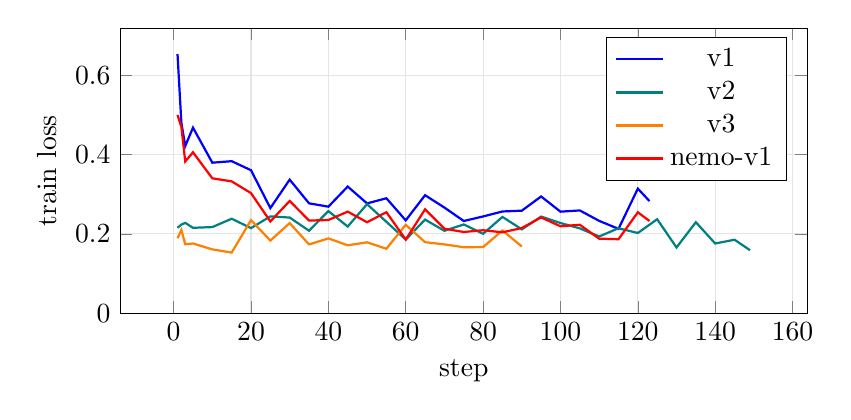
\begin{tikzpicture}
\begin{axis}[width=0.85\linewidth,height=5.2cm,xlabel={step},ylabel={train loss},legend pos=north east,grid=both,grid style={gray!20},ymin=0]
\addplot[blue,thick,mark=none] coordinates {(1,0.6532) (2,0.4798) (3,0.4213) (5,0.4678) (10,0.3794) (15,0.3832) (20,0.3604) (25,0.2649) (30,0.3367) (35,0.2769) (40,0.2685) (45,0.3192) (50,0.2767) (55,0.2897) (60,0.234) (65,0.2974) (70,0.2662) (75,0.2324) (80,0.2438) (85,0.2564) (90,0.2584) (95,0.2942) (100,0.2559) (105,0.259) (110,0.2327) (115,0.2125) (120,0.314) (123,0.2826)}; \addlegendentry{v1}
\addplot[teal,thick,mark=none] coordinates {(1,0.2151) (2,0.2233) (3,0.2276) (5,0.2152) (10,0.217) (15,0.2381) (20,0.2144) (25,0.244) (30,0.241) (35,0.2078) (40,0.2574) (45,0.2184) (50,0.2748) (55,0.2303) (60,0.1855) (65,0.2359) (70,0.2076) (75,0.2237) (80,0.2001) (85,0.2427) (90,0.2113) (95,0.2435) (100,0.2273) (105,0.2137) (110,0.1933) (115,0.214) (120,0.2021) (125,0.2368) (130,0.1656) (135,0.2293) (140,0.1756) (145,0.1851) (149,0.1587)}; \addlegendentry{v2}
\addplot[orange,thick,mark=none] coordinates {(1,0.1888) (2,0.2098) (3,0.1737) (5,0.1756) (10,0.1608) (15,0.1527) (20,0.2345) (25,0.1829) (30,0.2272) (35,0.1732) (40,0.1885) (45,0.171) (50,0.1786) (55,0.1624) (60,0.2228) (65,0.1789) (70,0.1734) (75,0.1662) (80,0.1666) (85,0.2085) (90,0.1681)}; \addlegendentry{v3}
\addplot[red,thick,mark=none] coordinates {(1,0.4998) (2,0.4693) (3,0.3826) (5,0.4056) (10,0.34) (15,0.3323) (20,0.3027) (25,0.2311) (30,0.283) (35,0.2334) (40,0.2349) (45,0.256) (50,0.2292) (55,0.2546) (60,0.1855) (65,0.2618) (70,0.2129) (75,0.2046) (80,0.2091) (85,0.2038) (90,0.2146) (95,0.2413) (100,0.2191) (105,0.2228) (110,0.1878) (115,0.1864) (120,0.2543) (123,0.2325)}; \addlegendentry{nemo-v1}
\end{axis}
\end{tikzpicture}
\end{center}
\noindent \textbf{Dev loss:} on a 96-sample dev set from the training writer, dev loss fell in v2 (0.269$\to$0.246), v3 (0.182$\to$0.151) and Nemotron (0.526$\to$0.210). One epoch per run. The model also holds up on calls from other writers (the Nemotron-written test set and the public BothBosu set).

\section{Evaluation protocol}
\begin{itemize}
\item \textbf{Streaming, the way the line runs it.} Each test call is scored turn by turn: the guardian sees the 8-turn window plus its own previous verdict, and scoring stops at its first alert.
\item \textbf{Metrics.}
\begin{itemize}
\item \textbf{Catch before ask} (headline): share of risky calls alerted \emph{before} the labeled ask turn (the request for the code, money, address, or meeting).
\item \textbf{False alarms}: share of benign calls (look-alikes included) that ever reach \emph{alert}.
\item \textbf{Rule-flip accuracy}: both members of a same-words / different-rules pair decided correctly.
\item Also: category macro-F1 at first alert, evidence-quote exact match, latency, and unparseable replies.
\end{itemize}
\item \textbf{Test sets.}
\begin{itemize}
\item \textbf{Held-out:} 257 Nemotron-written calls (148 with an ask turn, 79 benign, 22 rule-flip pairs).
\item \textbf{Held-out 120:} the first 120 held-out calls, scored for every system.
\item \textbf{BothBosu}~\cite{bothbosu}: public, LLM-written scam/non-scam conversations (out of distribution).
\item \textbf{ASR-50:} 49 held-out calls voiced with TTS, sent through 8\,kHz phone audio and transcribed by Nemotron Speech.
\end{itemize}
\item \textbf{Baselines.}
\begin{itemize}
\item B0: keyword rules.
\item B1: Rune (Fireworks' zero-shot decision model; yes/no ``alert now?'' plus category).
\item B3: the same Qwen3.6 base, untuned, with the same prompt.
\item B4: Kimi K3 (frontier).
\item B5: DeepSeek V4.1 Flash (frontier).
\end{itemize}
\end{itemize}

\section{Results}
\begin{table}[H]\centering\small
\caption{Same 120 held-out calls for every system.}\label{tab:t120}
\begin{adjustbox}{max width=\linewidth}\begin{tabular}{lcccc}\toprule
System & Catch before ask $\uparrow$ & False alarms $\downarrow$ & Rule-flip pairs $\uparrow$ & Cat.\ F1 \\ \midrule
B0 Keyword rules & 45.9\% \scriptsize(34/74; 35--57) & 41.7\% \scriptsize(15/36; 27--58) & 0/10 & 0.64 \\
B1 Rune (Fireworks, zero-shot) & 90.5\% \scriptsize(67/74; 82--95) & 33.3\% \scriptsize(12/36; 20--50) & 2/10 & 0.55 \\
B3 Qwen3.6-35B-A3B, untuned & 82.4\% \scriptsize(61/74; 72--89) & 55.6\% \scriptsize(20/36; 40--70) & 0/10 & 0.37 \\
B4 Kimi K3 (frontier) & 85.1\% \scriptsize(63/74; 75--91) & 25.0\% \scriptsize(9/36; 14--41) & 0/10 & 0.78 \\
B5 DeepSeek V4.1 Flash (frontier) & 81.1\% \scriptsize(60/74; 71--88) & 33.3\% \scriptsize(12/36; 20--50) & 1/10 & 0.53 \\
\midrule
\textbf{Ours: Qwen3.6 guardian v1} & 86.5\% \scriptsize(64/74; 77--92) & 16.7\% \scriptsize(6/36; 8--32) & 8/10 & 0.70 \\
\textbf{Ours: Qwen3.6 guardian v2} & 87.8\% \scriptsize(65/74; 78--93) & 25.0\% \scriptsize(9/36; 14--41) & 8/10 & 0.67 \\
\textbf{Ours: Qwen3.6 guardian v3} & 82.4\% \scriptsize(61/74; 72--89) & 13.9\% \scriptsize(5/36; 6--29) & 7/10 & 0.63 \\
\textbf{Ours: Nemotron 3.5 Super guardian} & 85.1\% \scriptsize(63/74; 75--91) & 13.9\% \scriptsize(5/36; 6--29) & 7/10 & 0.64 \\
\bottomrule\end{tabular}\end{adjustbox}
\par\smallskip\footnotesize Percent (count; 95\% Wilson interval).
\end{table}
\begin{table}[H]\centering\small
\caption{All 257 held-out calls (Nemotron-written).}\label{tab:t257}
\begin{adjustbox}{max width=\linewidth}\begin{tabular}{lcccc}\toprule
System & Catch before ask $\uparrow$ & False alarms $\downarrow$ & Rule-flip pairs $\uparrow$ & Cat.\ F1 \\ \midrule
B0 Keyword rules & 52.0\% \scriptsize(77/148; 44--60) & 49.4\% \scriptsize(39/79; 39--60) & 0/22 & 0.50 \\
B1 Rune (Fireworks, zero-shot) & 92.6\% \scriptsize(137/148; 87--96) & 38.0\% \scriptsize(30/79; 28--49) & 5/22 & 0.52 \\
B3 Qwen3.6-35B-A3B, untuned & 89.2\% \scriptsize(132/148; 83--93) & 53.2\% \scriptsize(42/79; 42--64) & 3/22 & 0.36 \\
B4 Kimi K3 (frontier) & 89.9\% \scriptsize(133/148; 84--94) & 22.8\% \scriptsize(18/79; 15--33) & 4/22 & 0.67 \\
B5 DeepSeek V4.1 Flash (frontier) & 85.1\% \scriptsize(126/148; 79--90) & 31.6\% \scriptsize(25/79; 22--43) & 3/22 & 0.52 \\
\midrule
\textbf{Ours: Qwen3.6 guardian v1} & 89.9\% \scriptsize(133/148; 84--94) & 16.5\% \scriptsize(13/79; 10--26) & 19/22 & 0.62 \\
\textbf{Ours: Qwen3.6 guardian v2} & 92.6\% \scriptsize(137/148; 87--96) & 17.7\% \scriptsize(14/79; 11--28) & 19/22 & 0.62 \\
\textbf{Ours: Qwen3.6 guardian v3} & 86.5\% \scriptsize(128/148; 80--91) & 12.7\% \scriptsize(10/79; 7--22) & 18/22 & 0.66 \\
\textbf{Ours: Nemotron 3.5 Super guardian} & 89.2\% \scriptsize(132/148; 83--93) & 15.2\% \scriptsize(12/79; 9--25) & 17/22 & 0.55 \\
\bottomrule\end{tabular}\end{adjustbox}
\par\smallskip\footnotesize Percent (count; 95\% Wilson interval).
\end{table}

\begin{table}[H]\centering\small
\caption{The gain is real. Guardian v2 against every system on all 257 held-out calls. A call is \emph{handled} when a risky call is alerted before its ask (or at all, when it has none) or a harmless call is never alerted. Wins / losses = calls only one of the two handled. McNemar's exact test on those disagreements; 95\% interval from 5,000 bootstrap resamples of whole scenarios (73 clusters), since calls from one scenario share a script.}\label{tab:sig}
\begin{adjustbox}{max width=\linewidth}\begin{tabular}{lrrrrr}\toprule
Guardian v2 (90.3\% handled) vs. & Their handled & Gain & Wins / losses & McNemar $p$ & Bootstrap 95\% interval \\ \midrule
B3 Qwen3.6-35B-A3B, untuned & 75.5\% & +14.8 pts & 40 / 2 & $4\times10^{-10}$ & +8.9 to +20.9 \\
B5 DeepSeek V4.1 Flash & 79.4\% & +10.9 pts & 33 / 5 & $4\times10^{-6}$ & +4.9 to +16.6 \\
B1 Rune (Fireworks) & 83.3\% & +7.0 pts & 28 / 10 & 0.005 & +1.7 to +12.0 \\
B4 Kimi K3 & 83.7\% & +6.6 pts & 24 / 7 & 0.003 & +0.9 to +12.3 \\
B0 Keyword rules & 54.5\% & +35.8 pts & 100 / 8 & $2\times10^{-21}$ & +27.3 to +43.7 \\
\bottomrule\end{tabular}\end{adjustbox}\end{table}

\begin{table}[H]\centering\small
\caption{Routing across models: Rune as a 0.15\,s first-pass gate, our guardian confirms before the caretaker is alerted (computed from cached per-turn predictions; risk is monotonic within a call).}\label{tab:cascade}
\begin{adjustbox}{max width=\linewidth}\begin{tabular}{lcccc}\toprule
& \multicolumn{2}{c}{All 257 held-out} & \multicolumn{2}{c}{Same 120} \\ \cmidrule(lr){2-3}\cmidrule(lr){4-5}
Cascade & Catch before ask & False alarms & Catch before ask & False alarms \\ \midrule
Rune $\rightarrow$ \textbf{Ours: Qwen3.6 guardian v1} & 87.8\% (130/148) & 10.1\% (8/79) & 85.1\% (63/74) & 8.3\% (3/36) \\
Rune $\rightarrow$ \textbf{Ours: Qwen3.6 guardian v2} & 89.9\% (133/148) & 10.1\% (8/79) & 85.1\% (63/74) & 11.1\% (4/36) \\
Rune $\rightarrow$ \textbf{Ours: Qwen3.6 guardian v3} & 85.1\% (126/148) & 10.1\% (8/79) & 81.1\% (60/74) & 11.1\% (4/36) \\
Rune $\rightarrow$ \textbf{Ours: Nemotron 3.5 Super guardian} & 87.8\% (130/148) & 11.4\% (9/79) & 83.8\% (62/74) & 8.3\% (3/36) \\
\bottomrule\end{tabular}\end{adjustbox}\end{table}

\begin{table}[H]\centering\small
\caption{Out of distribution: BothBosu (written by a different model family; call-level labels, so catch-before-ask does not apply).}\label{tab:bb}
\begin{tabular}{lcc}\toprule System & Scam recall & False alarms \\ \midrule
B0 Keyword rules & 43\% (43/100) & 0/100 \\
\textbf{Ours: Qwen3.6 guardian v1} & 95\% (95/100) & 0/100 \\
\textbf{Ours: Qwen3.6 guardian v2} & 98\% (98/100) & 0/100 \\
\textbf{Ours: Qwen3.6 guardian v3} & 97\% (97/100) & 0/100 \\
\textbf{Ours: Nemotron 3.5 Super guardian} & 100\% (100/100) & 0/100 \\
\bottomrule\end{tabular}\end{table}

\begin{table}[H]\centering\small
\caption{Real speech recognition: the same 49 held-out calls as clean text vs.\ TTS $\to$ 8\,kHz $\to$ Nemotron Speech ASR (median WER 15.9\%, mean 24.5\%, mostly numbers written as words).}\label{tab:asr}
\begin{adjustbox}{max width=\linewidth}\begin{tabular}{lccccc}\toprule
& \multicolumn{2}{c}{Clean text} & \multicolumn{2}{c}{ASR text} & \\ \cmidrule(lr){2-3}\cmidrule(lr){4-5}
System & Catch & FA & Catch & FA & Risky flagged at all (ASR) \\ \midrule
B1 Rune (Fireworks, zero-shot) & 88.9\% & 3/16 & 88.9\% & 2/16 & 97\% \\
B5 DeepSeek V4.1 Flash (frontier) & 81.5\% & 4/16 & 85.2\% & 5/16 & 97\% \\
\textbf{Ours: Qwen3.6 guardian v1} & 85.2\% & 1/16 & 81.5\% & 3/16 & 100\% \\
\textbf{Ours: Qwen3.6 guardian v2} & 85.2\% & 4/16 & 85.2\% & 2/16 & 100\% \\
\bottomrule\end{tabular}\end{adjustbox}
\par\smallskip\footnotesize Nothing collapses on real transcripts: v1 and v2 still flag every risky call.
\end{table}

\subsection*{Key findings}
\begin{enumerate}
\item \textbf{Fine-tuning works.} The same base model untuned false-alarms on 53.2\% of harmless calls and gets 3/22 rule pairs; fine-tuned v2 gets 17.7\% and 19/22, with more early catches (92.6\% vs.\ 89.2\%). The gain is significant ($p = 4\times10^{-10}$; Table~\ref{tab:sig}).
\item \textbf{Beats the frontier models.} On all 257 held-out calls, v2 handles 90.3\% of calls against 83.7\% for Kimi K3, 83.3\% for Rune and 79.4\% for DeepSeek V4.1 Flash, each significant under both tests. It has fewer false alarms than every baseline and follows caretaker rules the frontier models miss (19/22 vs.\ 3--5/22).
\item \textbf{A tunable operating point.} v3 reaches the fewest false alarms of any single model (12.7\%); routing Rune$\rightarrow$guardian reaches about 10\% false alarms at frontier-level catch.
\item \textbf{Holds up when the writer and the audio change.} 95--100\% scam recall with zero false alarms on BothBosu, and v1/v2 still flag every risky call on real Nemotron Speech transcripts.
\end{enumerate}

\section{Team}
\begin{itemize}
\item \textbf{Numan Karakas}: the phone line (Telnyx call flow, conference coach line, caretaker alert call), Nemotron Speech integration, the console backend, the Google Cloud jobs and the AI-voice detector.
\item \textbf{Matt Ceran}: the guardian model (scenario taxonomy, data factory, fine-tuning, evaluation, baselines) and the caretaker console.
\end{itemize}

\section{The NVIDIA thread}
NVIDIA models carry three jobs:
\begin{itemize}
\item \textbf{Nemotron Speech Streaming 0.6B} hears every live call on a laptop.
\item \textbf{Nemotron 3 Ultra} wrote the held-out test set.
\item A \textbf{fine-tuned Nemotron 3.5 Super} guardian (same data as v1) catches 89.2\% before the ask with 15.2\% false alarms, gets 17/22 rule pairs, and hits 100\% BothBosu recall with 0 false alarms.
\end{itemize}


\begin{thebibliography}{9}\small
\bibitem{ic3} Federal Bureau of Investigation, Internet Crime Complaint Center. \emph{2025 IC3 Annual Report}. \url{https://www.ic3.gov/AnnualReport/Reports/2025_IC3Report.pdf}
\bibitem{ftc} Federal Trade Commission. \emph{FTC data show people reported losing \$3.5 billion to imposter scams in 2025}. Press release, June 2026. \url{https://www.ftc.gov/news-events/news/press-releases/2026/06/ftc-data-show-people-reported-losing-3-point-5-billion-imposter-scams-2025}
\bibitem{ncmec} National Center for Missing \& Exploited Children. \emph{CyberTipline data}. \url{https://www.missingkids.org/cybertiplinedata}
\bibitem{bothbosu} BothBosu. \emph{Scammer-Conversation} dataset (Apache-2.0). \url{https://huggingface.co/datasets/BothBosu/Scammer-Conversation}
\bibitem{itw} N.~M. M\"uller, P.~Czempin, F.~Dieckmann, A.~Froghyar, K.~B\"ottinger. \emph{Does Audio Deepfake Detection Generalize?} Interspeech 2022 (In-the-Wild dataset). \url{https://arxiv.org/abs/2203.16263}
\bibitem{nemospeech} NVIDIA. \emph{Nemotron Speech Streaming 0.6B (English)}. \url{https://huggingface.co/nvidia/nemotron-speech-streaming-en-0.6b}
\bibitem{fwtapi} Fireworks AI. \emph{Serverless Training} (Training API documentation). \url{https://docs.fireworks.ai/fine-tuning/training-api/serverless}
\end{thebibliography}

\appendix
\section{Reference}
\sloppy
\begin{itemize}
\item \textbf{Repository:} \url{https://github.com/matt-ceran/fireworks-AMD} (branch \texttt{main}).
\item \textbf{Checkpoint:} \path{afceran33-zaqel7a5ap/run-d0f99835415b46f5a898cafaa544e005/v2-fin-7ecb9b48}. Promoted model: \path{accounts/afceran33-zaqel7a5ap/models/emberz-guardian-v2}.
\item \textbf{Code} (all under \path{callguard/}):
  \begin{itemize}
  \item prompt contract: \path{guardian/render.py} (prompt\_sha \texttt{806908cfba7d})
  \item training: \path{guardian/train_tapi.py}
  \item evaluation: \path{eval/run_eval.py}
  \item serving the evaluated checkpoint: \path{guardian/sampler_proxy.py}
  \item caretaker console: \path{console/}
  \end{itemize}
\item \textbf{Live phone line} (repo root): \path{line/}; AI-voice detector: \path{voice/}; one-command demo: \path{demo/run_demo.sh}.
\end{itemize}

\section{The live line works on real phone calls}
On November 2, 2026 we called the guarded Telnyx number with an AI bank-scam caller (an LLM script with a neural TTS voice over SignalWire, about \$0.34 per two-minute call) and bridged it to a real phone. Logs: \path{results/ledger-numan.md}; recordings: \path{recordings/}.
\begin{itemize}
\item \textbf{15:11 PST.} Both sides were transcribed live (11 turns). The guardian raised an \emph{urgent} alert on the bank impersonation (turn 4) and again on the request for the verification code (turn 10). Three coach lines went to the protected leg only, 0.70--0.75\,s after the turn that triggered them; the caller heard nothing. The caretaker was phoned at the first alert, pressed 1, joined in listen-only mode and heard the second alert whispered.
\item \textbf{15:48 PST, on the exact evaluated checkpoint} (served through \path{sampler_proxy.py}). Urgent alerts at 58\,s and 83\,s, a coach line, and the caretaker listening. The caretaker then \textbf{pressed 9}: Emberz dropped the scam caller, told the protected person ``you are safe'', and ended the call.
\item \textbf{AI voice, live.} On 5 live calls our detector flagged the synthetic caller 4 times (scores 0.96--0.9995 for Azure and Google voices) and missed one Cartesia voice (0.41). This is a small sample, not a benchmark; Table~2 is the benchmark.
\item \textbf{Never left unguarded.} If the guardian endpoint is down (for example, a deployment scaled to zero), the line scores turns with NVIDIA Nemotron Lightning~3.5 on Fireworks serverless instead.
\end{itemize}
\end{document}
